\documentclass[11pt]{article}
\usepackage[margin=1in]{geometry}
\usepackage{amsmath,amssymb}
\usepackage{booktabs}
\usepackage{graphicx}
\usepackage{hyperref}
\usepackage{caption}
\usepackage{float}
\hypersetup{colorlinks=true,linkcolor=blue,citecolor=blue,urlcolor=blue}

\title{A finite-integer causal-lattice testbed:\\
which resources reproduce interference, causal collapse\\
and Bell correlations on one lattice}
\author{Alon Gonen\\
\small Independent researcher\\
\small \texttt{alon@defounder.ai} \quad ORCID 0009-0008-2701-4599}
\date{September 2026}

\begin{document}
\maketitle

\begin{abstract}
We describe Universe24, a simulator in which space is a three-dimensional
lattice of Nodes joined by six Links, every evolving quantity is a bounded
integer, and every rule is local, and we use it as a testbed: several
candidate microscopic mechanisms run under identical computational
conditions, and the question asked of each is which resource it needs to
reproduce a given correlation. The mechanisms are a classical phased-ray
field, a finite quantum owner (a joint state over at most thirty registers
with Gaussian-integer unitaries and Kraus instruments), a causal source
candidate that couples the two through a local envelope rule, and a bonded
pair whose joint outcome is answered by one shared registry. The laws each
mechanism obeys (mixers, phase advance, the cosine table, the singlet law)
are configured inputs, not derived; the measurements verify that the
implementation realizes them exactly in bounded integers and record what
finite causal delay does to them. On the canonical runner we record exact
rational interference weights, which-path decoherence by a local instrument,
a collapse that reaches remote sources only after Link transit, a local
null-notice rule that restores conditional Born weights after one Link and
corrects crossing nulls, an external-field phase, an emission-side energy
closure and the emission-side classical limit. We then run the CHSH form of
Bell's test on every candidate. The three candidates whose information
travels only on Links give $S = 1.40$ (exact), $1.38$ and exactly $2$; the
plain field gives exactly $2$; the two candidates with one shared object give
$S = 2.84 \pm 0.02$ (the bonded pair, 4096 fresh pairs per correlation,
four replicas; the registry alone gives $2.827 \pm 0.001$ at a million pairs,
its exact expectation on the integer cosine table being $724/256 = 2.828$)
and $S = 14/5$ (the quantum owner at 3-4-5 settings). For each candidate we identify, by
measurement at fixed hidden variable, which assumption of Bell's theorem it
breaks: the bonded pair is deterministic and measurement-independent and
breaks parameter independence, the quantum owner breaks outcome independence,
and the local candidates break none. A no-signalling check on the number
source is reported and distinguished from locality. Nothing here derives
quantum mechanics or explains the Bell value locally; the contribution is a
reproducible integer framework in which the causal assumptions behind Bell's
theorem, and the cost of finite causal delay, appear as measured tables.
The code base is published as Reality Theory (Universe24).
\end{abstract}

\section{Introduction}

Discrete, local, integer models of physics have a long history: conservative
logic and cellular automata \cite{fredkin1982,thooft2016}, lattice gases
\cite{fhp1986,succi2001}, quantum cellular automata and quantum lattice gases
\cite{bialynicki1994,meyer1996,arrighi2019}, hybrid quantum--classical
dynamics \cite{rosenfeld1963,diosi1984,oppenheim2023}, collapse and
decoherence \cite{grw1986,bassi2013,zurek2003}, and histories and causal sets
\cite{griffiths1984,bombelli1987}. Bell's theorem and its causal anatomy are
equally settled \cite{bell1964,chsh1969,jarrett1984,shimony1986,hall2010}:
a model that keeps measurement independence and factorizes as
$P(A,B|a,b,\lambda) = P(A|a,\lambda)\,P(B|b,\lambda)$ satisfies $S \le 2$,
and every model above the bound gives up a named assumption. This paper
claims none of these results as new.

What it reports is a testbed. Universe24 runs classical fields, a finite
quantum state, a hybrid coupling and a shared-registry pair on one lattice,
under one scheduler, with one arithmetic (bounded integers), one causal rule
(one Link per tick) and one audit (per-event conservation). Because the
candidates share everything except the resource under test, the same
experiment can be run on each of them and the differences attributed to that
resource. The paper asks three questions of this kind. Which candidates
reproduce two-path interference, and with which configured inputs? What does
a finite causal delay do to conditional collapse, and can a local rule repair
it? And, for Bell's test, which resource each candidate needs to reach its
$S$, stated as the assumption of Bell's theorem it breaks and measured rather
than argued.

Two disclaimers frame every table. First, the laws are inputs. The mixers,
the instruments, the phase advance, the cosine table and the singlet law in
the registry are configuration data; a curve that follows $(1-\cos\phi)/2$
verifies that the integer implementation realizes the configured law
exactly, and nothing more. Second, the candidate that exceeds the Bell bound
does so through a declared shared object; it is not a local explanation of
the quantum correlations, and Section~\ref{sec:causal} says precisely which
assumption it gives up.

Section~\ref{sec:model} states the model and its inputs.
Section~\ref{sec:coupling} reports the coupling experiments.
Section~\ref{sec:bell} reports Bell's test on every candidate with its
statistics, Section~\ref{sec:causal} the causal analysis, and
Section~\ref{sec:outside} the no-signalling check on the number source.
Section~\ref{sec:new} states what is new and Section~\ref{sec:notclaimed}
what is not claimed. All code, configurations and recorded runs are archived
\cite{zenodo}.

\section{The model and its inputs}\label{sec:model}

\paragraph{Lattice and locality.} Nodes lie on a three-dimensional integer
lattice with open or periodic boundary; each Node has six Links. One tick
moves a packet across one Link. A Node's state is a fixed set of bounded
integer registers; there is no global variable that a physical rule reads.
Postulate 4 states the causal bound: energy, momentum, matter and every
message a record can control move at most one Node per step. The bond
registry of the last paragraph below is the one declared exception.

\paragraph{Integers.} Every physical quantity, intermediate and law table is
a bounded integer or a ratio of bounded integers; there is no floating point
in any physical module, and an audit test enforces it. Trigonometric tables
for phased rays are prepared once in fixed point (scale 256) with a bounded
series.

\paragraph{Computation cost and delay.} Every local cycle has a cost in
configured operation prices, and a cycle whose cost exceeds the normal budget
$B$ delays its Node by $\lceil C/B \rceil$ intervals; Link transit stays one
tick and no debt accumulates. A configured conserved field may be named the
computation field, so that a mass which emits it slows the carriers that
pass it; with directional delay each departure waits for the load on its
channel, and with least-delay routing every carrier takes the cheapest
eligible port first while keeping exact directional ratios. These are declared
timing rules, not a gravitational law; their measured consequences (a pulse
that does not cross a loaded region within the run, a fringe shifted by the
waits beside a mass, a distance-proportional redshift on a closed lattice
whose load grows with age) are recorded in the archive and not used here.

\paragraph{Classical disturbances and fields.} Records with configured fields
move and interact by local rules. Spatial fields are transported by an octant
rule or by straight rays that keep one integer line, one Link per tick, and
are counted whole by the ledger. Ray emission may be funded from the
emitter's stock, with recoil; absorption adds the ray's amount and momentum
to the absorber. A local conservation audit closes energy and momentum per
event.

\paragraph{Phased rays.} A ray field may carry a phase step per ray, advanced
once per Link; rays meeting at a Node combine by the fixed-point cosine of
their phase differences, and the coherence
$|\sum a e^{i\phi}|^2 / (\sum |a|)^2$ gates what a reader samples and what an
absorber takes. Capture is a run-time choice: the coherent share, a whole-ray
lottery drawn from a record-row ticket, a deterministic threshold, or, for
bonded pairs, an answer of the bond registry.

\paragraph{The finite quantum owner.} A domain of at most thirty registers
holds a joint state with Gaussian-integer amplitudes. Gates are local
unitaries $U$ with $U^\dagger U = s I$ for an integer scale $s$; instruments
are Kraus pairs $(sI + O, sI - O)$; decisions carry exact rational Born
weights, and a ticket selects an outcome only when more than one weight is
nonzero. The Born weights are a configured reading of the state, not a
derived one.

\paragraph{The causal source candidate.} At an actual local contact a record
becomes a unit source envelope: a bounded complex amplitude at that Node.
Two-mode gates between neighboring Nodes exchange frozen amplitudes through
Links and commit after the neighbor's packet arrives. Each Node emits the
ordinary classical field at the configured full strength times its local
squared magnitude. A capture localizes the excitation into an ordinary record
and sends a terminal notice through Links; remote envelopes stop when it
arrives. A null result zeros only the local envelope; with the opt-in null
notice the deciding Node sends its own factor $1/(1-p)$ through Links, and a
Node whose own null was decided before an earlier-ordered notice arrived
answers with the exact correction $(1 - w s)/(1 - w s g)$ from its own record.

\paragraph{Bonded pairs and the registry.} Two rays emitted together carry
the code of their birth Node and tick. A detector meeting a bonded ray asks
the bond registry, one bounded object for the world (at most 4096 open pairs,
each released at its second answer, repeated questions idempotent). The
pair's one number $\lambda$ is a fixed function of the registry seed and the
birth code, chosen before any setting exists. Its upper half answers the
first end evenly; its lower half, read against the difference of the two
settings, decides whether the second end agrees, with probability
$(1 - \cos(a-b))/2$ taken from the cosine table. The second answer therefore
reads the first end's setting. The registry moves no energy, momentum or
inventory, and each end alone sees an even coin; Section~\ref{sec:causal}
states what this does and does not buy.

\paragraph{One integer per interaction (postulate 22).} Every interaction
whose outcome is not certain consumes exactly one bounded integer from a
configured sequence: the record's ticket, the quantum owner's ticket, or the
registry's number. The world's history is fixed by the rules, the initial
state and this sequence, and the sequence is the only place where information
not in the world's state enters. The model does not fix the generator of the
sequence, but it does fix how each number is read, and that decides which
assumption of Bell's theorem is at stake. A number chosen before the settings
and read by one end only is a local hidden variable (the lottery ticket) and
keeps $S \le 2$. A number chosen before the settings and read by both ends
(the registry) keeps measurement independence and gives up parameter
independence. A number correlated with the settings would relax measurement
independence \cite{hall2010}; no rule in the model does that, and no claim
about such a source is made. Whatever supplies the numbers is also bound by
no-signalling, which Section~\ref{sec:outside} measures; no-signalling is a
weaker condition than locality and is not offered as one.

\section{Coupling experiments}\label{sec:coupling}

All runs use the canonical headless runner on a $7\times3\times3$ open world
with one domain of three registers $S=(1,1,1)$, $M=(2,1,1)$, $D=(3,1,1)$, a
$3{:}4$ mixer with amplitudes $(3/5, 4/5)$, a one-mode phase gate on $M$, the
inverse mixer, and a SWAP to $D$ where a held probe attempts capture. Analytic
targets are computed independently of the update code. Every row of
Table~\ref{tab:coupling} is a verification that the integer implementation
realizes its configured law exactly; the null-notice, crossing-null and
Link-transit rows are in addition results about finite causal delay, which
the configured laws do not fix.

\begin{table}[h]\centering\small
\resizebox{\linewidth}{!}{\begin{tabular}{lll}
\toprule
Observation & Result & Prediction\\
\midrule
Capture weights at $D$, $\phi=0,\pi/2,\pi,3\pi/2$ & $[625,0],[337,288],[49,576],[337,288]$ & $288(1-\cos\phi)/625$ exact\\
Balanced Hadamard splitter (vacuum $1+i$) & capture probability $0,\tfrac12,1,\tfrac12$ & exact\\
Classical emission at $S$ after recombination & $25, 13.5, 2, 13.5$ per tick & $\lfloor 25(337+288\cos\phi)/625\rfloor$ with carry\\
Held detector on the arm & $[9,16]$ for every $\phi$; no capture at $D$ & which-path\\
Capture two Links away & $S$ emits once more, then stops & Link transit\\
Null notice after an arm null & $S$ emits $25/25$ from the next tick; next gate $9$ and $16$ & conditional Born weights\\
Crossing nulls on one tick & stale product $390625/177489$; corrected to $25/9$ at every Node & exact conditional scale\\
External field phase, coil $0,200,400,800$ & exponents $0,0,1,2$; capture $0, 0, 576/3125, 9216/15625$ & $144((a-5^n)^2+b^2)$\\
Funded emission, stock 3000 & totals constant; paid 211 (null) / 199 (capture); residual 2 & emission-side closure\\
Emission scale $25\to25000$ & departure $<1$ unit per tick; exact at multiples of 625 & $\text{amount}\times|\psi|^2$\\
\bottomrule
\end{tabular}}
\caption{Coupling measurements on the canonical runner. Every recorded weight equals the exact rational prediction of the configured law.}
\label{tab:coupling}
\end{table}

Three rows deserve a sentence each. The which-path row is decoherence by an
actual local instrument using only local state and Link-delivered inputs.
The null-notice rows show that, for one excitation, the retarded local
approximation can be made exact by a factor known at the null Node, at the
cost of Link transit, and that two nulls crossing in flight are corrected
locally by the later Node; the stale emission in between is the candidate's
causal residual, a property of finite delay rather than an error. The
emission-scale row is the classical limit on the emission side only: the
integer field becomes the continuous law, while the wave's own dynamics stay
configured.

\begin{figure}[h]\centering
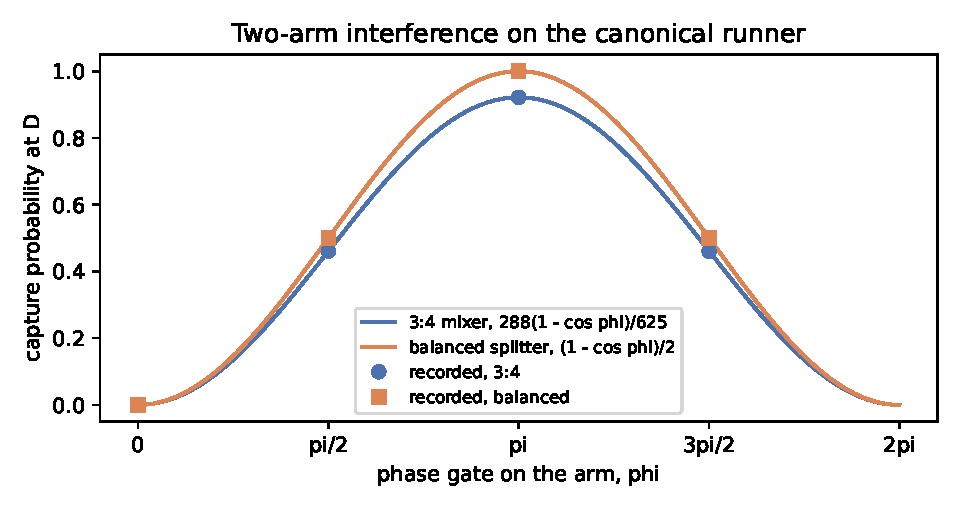
\includegraphics[width=0.85\linewidth]{figures/interference.pdf}
\caption{Capture probability at $D$ against the arm phase for the $3{:}4$ mixer and the balanced splitter; curves are the exact rational predictions of the configured mixers, points the recorded decision weights.}
\end{figure}
\begin{figure}[h]\centering
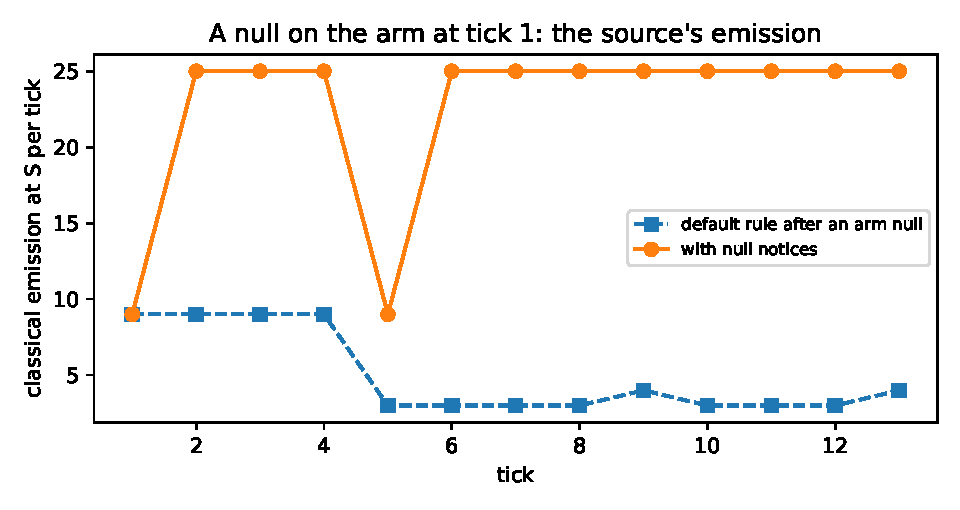
\includegraphics[width=0.48\linewidth]{figures/null_notices.pdf}\hfill
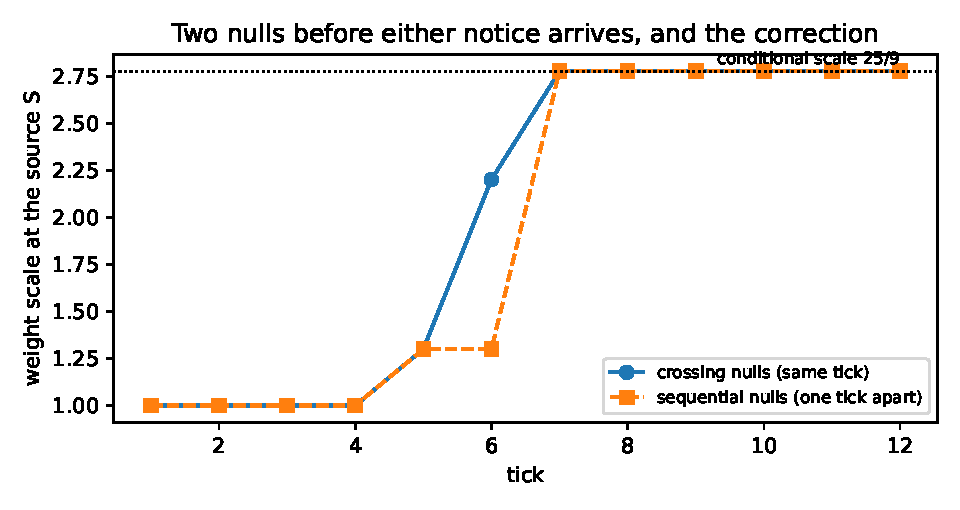
\includegraphics[width=0.48\linewidth]{figures/crossing_nulls.pdf}
\caption{Left: the source's classical emission per tick after an arm null at tick 1, under the default retarded rule and with null notices; the notice restores $25/25$ one Link later and the next gate emits the conditional weights. Right: the weight scale at the source when two nulls cross in flight and when they are sequential; the later Node's correction brings both to the conditional scale $25/9$.}
\end{figure}
\begin{figure}[h]\centering
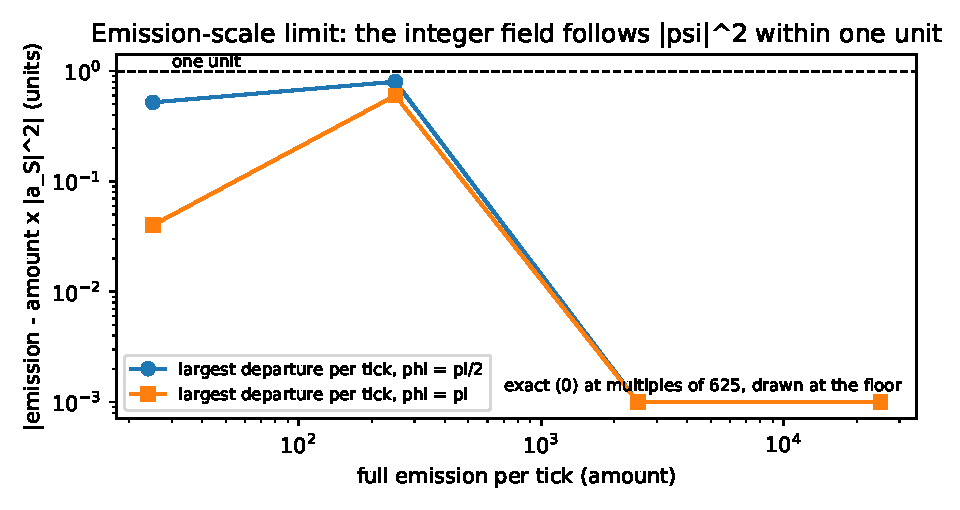
\includegraphics[width=0.85\linewidth]{figures/scale.pdf}
\caption{Largest per-tick departure of the classical emission from $\mathrm{amount}\times|a_S|^2$ as the full emission grows; below one unit at every scale and exactly zero at multiples of 625.}
\end{figure}

\section{Bell's test on every candidate}\label{sec:bell}

We run the CHSH form, $S = |E(a,b) - E(a,b') + E(a',b) + E(a',b')|$, on two
probes. The phased-ray probe uses the quantum owner's settings, Alice $Z$ or
$X$ and Bob $(3Z \pm 4X)/5$, read as phases $0^\circ, 90^\circ, 53^\circ,
307^\circ$ on a 360-step circle; the quantum value at these settings is
$14/5$. The ray Bell probe uses the optimal settings $0^\circ, 90^\circ,
45^\circ, 135^\circ$ on a 64-step circle, whose quantum value is $2\sqrt2$;
on that circle the table cosine of $45^\circ$ is $181/256$, so the exact
expectation of a mechanism obeying the table's singlet law is
$4 \times 181/256 = 724/256 = 2.828125$. The reading of a measurement
setting as a phase on the ray field is a configured correspondence. Each row
of Table~\ref{tab:bell} is compared with the quantum value at its own
settings; where a value is a count, its binomial standard error is given.

\begin{table}[H]\centering\footnotesize\setlength{\tabcolsep}{4pt}
\begin{tabular}{p{3.0cm}p{4.5cm}p{2.6cm}p{4.6cm}}
\toprule
Candidate & What decides the outcome & Settings (quantum $S$) & $S$\\
\midrule
Phased rays, share rule & coherent share against a local reference & 3-4-5 ($14/5$) & $826177/589824 = 1.4007$, exact\\
Phased rays, lottery & a local ticket at the coherent rate & 3-4-5 ($14/5$) & $386/279 = 1.38 \pm 0.04$ (2232 pairs; $1.40$ predicted)\\
Phased rays, threshold & deterministic: the whole ray when the share reaches $\tfrac12$ & $45^\circ$ ($2\sqrt2$) & $2.00$, exact\\
Plain rays, no phase & every ray absorbed whole & 3-4-5 ($14/5$) & $2$, exact\\
Bonded rays & the bond registry, one number per pair & $45^\circ$ ($2\sqrt2$; table $724/256$) & $2.837 \pm 0.015$ (4096 pairs per correlation, 4 replicas)\\
Bonded rays, registry alone & the same law without the lattice & $45^\circ$ & $2.8269 \pm 0.0010$ ($10^6$ pairs, 4 replicas)\\
Finite quantum owner & the joint conditional state at each contact & 3-4-5 ($14/5$) & $14/5$, exact; dephased control $6/5$\\
\bottomrule
\end{tabular}
\caption{One lattice, one runner, each candidate against the quantum value at its own settings; where a value is a count, its binomial standard error follows it. Candidates whose information travels only on Links stay at or below 2; the two with one shared object reach the quantum value at their settings.}
\label{tab:bell}
\end{table}

\paragraph{Statistics of the bonded value.} The first bonded run, 1024 pairs
per correlation with the four setting pairs sharing the same registry
numbers, read $S = 2.889$; its four correlations were not independent
samples, and a bar above $2\sqrt2$ would have been misleading without an
error. We therefore re-measured with fresh pairs for every setting pair, at
64, 256, 1024 and 4096 pairs per correlation on the lattice with four
independent replicas at each size, and with the registry alone (the same
seeds, no lattice) up to $10^6$ pairs. Every lattice outcome equals the
registry's answer from the same seed, pair by pair (87,040 of 87,040),
which states in one number where the Bell value lives: in the registry's
law, with the lattice adding transport and nothing else. Figure~\ref{fig:conv}
shows the convergence to the table expectation $724/256$; at 4096 pairs the
mean of four lattice replicas is 2.837 with an error of the mean of
0.015 (binomial prediction 0.011) and replica spread 0.030, and at $10^6$ registry
pairs it is 2.8269 $\pm$ 0.0010. The excess of the first run
was sampling. One property of the world's sequence shows in the replicas: it
is a polynomial congruence, not a random source, and replicas drawn from
consecutive seed blocks vary less than a random sample at small counts (a
spread of 0.003 against a binomial 0.044 at 1000 registry pairs); the mean
settles on the expectation only above $10^5$ pairs.

\begin{figure}[H]\centering
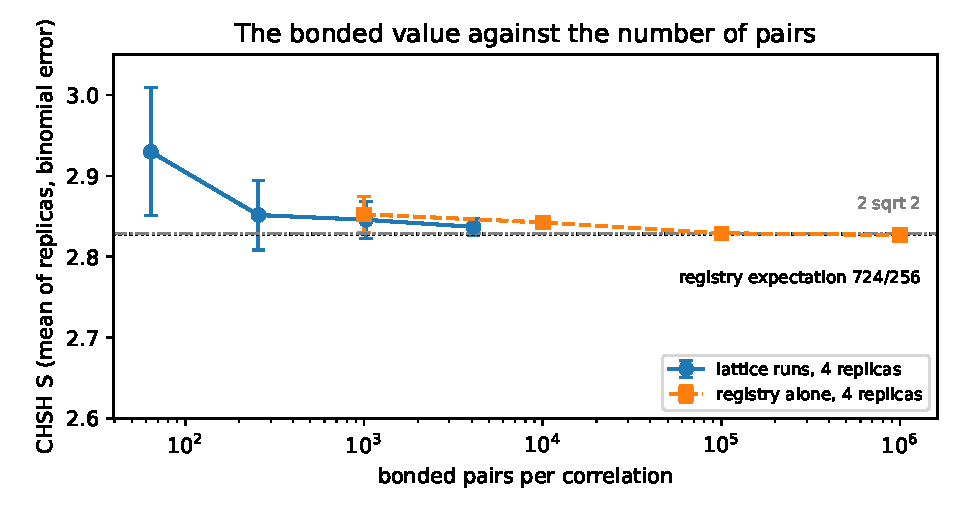
\includegraphics[width=0.85\linewidth]{figures/bond_convergence.pdf}
\caption{The bonded CHSH value against the number of pairs per correlation, on the lattice and with the registry alone; error bars are the binomial standard error of the mean of four replicas. The value converges to the registry's expectation $724/256$, three parts in ten thousand below $2\sqrt2$ because the cosine table holds $181/256$; the local bound 2 lies below the frame.}
\label{fig:conv}
\end{figure}

\begin{figure}[h]\centering
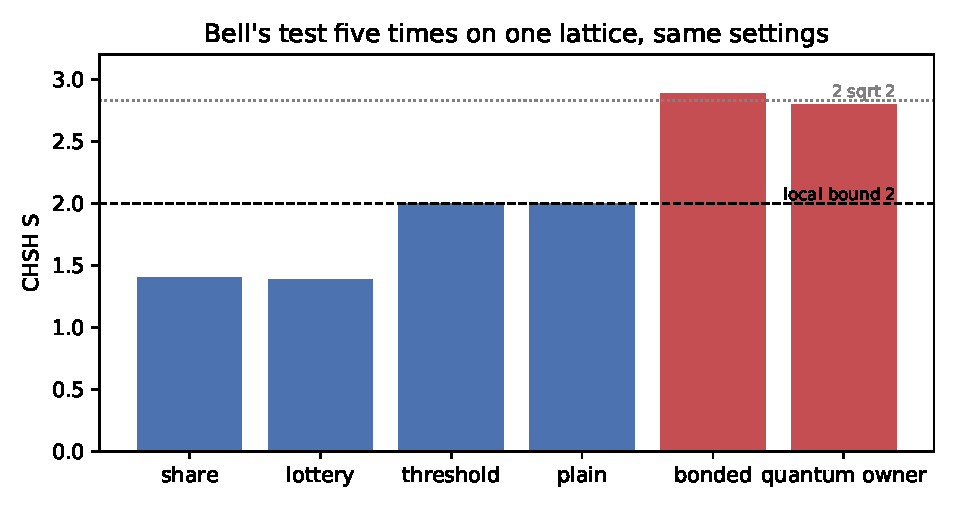
\includegraphics[width=0.85\linewidth]{figures/bell_candidates.pdf}
\caption{The Bell candidates and the plain field on one lattice, with binomial errors where a value is a count. Blue: information travels only on Links. Red: one shared object no Link carries.}
\end{figure}

\section{Which assumption of Bell's theorem each candidate breaks}\label{sec:causal}

Write $\lambda$ for everything fixed before the settings are chosen, $a, b$
for the settings, $A, B \in \{\pm1\}$ for the outcomes. Bell locality is the
factorization
\begin{equation}
P(A,B\,|\,a,b,\lambda) = P(A\,|\,a,\lambda)\,P(B\,|\,b,\lambda),
\label{eq:factor}
\end{equation}
which Jarrett and Shimony split into parameter independence,
\begin{equation}
P(A\,|\,a,b,\lambda) = P(A\,|\,a,\lambda), \qquad P(B\,|\,a,b,\lambda) = P(B\,|\,b,\lambda),
\label{eq:pi}
\end{equation}
and outcome independence, $P(B\,|\,a,b,\lambda,A) = P(B\,|\,a,b,\lambda)$
\cite{jarrett1984,shimony1986}; measurement independence is
$\rho(\lambda\,|\,a,b) = \rho(\lambda)$. With all three, $S \le 2$
\cite{chsh1969}. Because every candidate here is a program, each of these
conditions can be measured rather than argued: we fix $\lambda$, run the four
setting pairs, and count how often an outcome changes when only the other
end's setting changes.

For the phased-ray candidates $\lambda$ is the hidden phase and the
detectors' seed; for the bonded pair it is the registry's number, a function
of the seed and the birth code; for the quantum owner it is the prepared
joint state. In every case $\lambda$ is chosen before the settings and no
rule reads the settings when choosing it, so measurement independence holds
by construction; the probe also confirms that the same registry number serves
every setting pair. Table~\ref{tab:causal} gives the measured rates over 256
hidden variables (64 hidden phases, four seeds) per candidate.

\begin{table}[H]\centering\footnotesize\setlength{\tabcolsep}{4pt}
\begin{tabular}{p{2.1cm}p{2.2cm}p{2.0cm}p{4.1cm}p{2.9cm}l}
\toprule
Candidate & $\lambda$ & Measurement indep. & Parameter independence & Outcome independence & $S$\\
\midrule
Lottery & hidden phase, detector seed & by construction & holds: no outcome moves, 0 of 256 at either end & holds: two independent tickets & $1.38$\\
Threshold & hidden phase & by construction & holds: 0 of 256 at either end & holds: deterministic & $2$\\
Bonded pair & the registry's number & by construction & \textbf{broken}: $A$ never moves with $b$; $B$ moves with $a$ for 184 of 256 at $b'$ ($0.72$; law $362/512 = 0.707$) & holds: $A, B$ are functions of $\lambda$ and the settings & $2.83$\\
Quantum owner & the joint state & holds & holds: each marginal is the state's & \textbf{broken}: the joint conditional state & $14/5$\\
\bottomrule
\end{tabular}
\caption{The causal anatomy of every candidate, measured at fixed hidden variable over 256 hidden variables. A local candidate never moves an outcome with the other end's setting; the bonded pair moves Bob's outcome with Alice's setting, which is parameter dependence; the quantum owner keeps parameter independence and breaks outcome independence, as quantum mechanics does.}
\label{tab:causal}
\end{table}

The bonded pair is therefore a deterministic, measurement-independent,
parameter-dependent model, in the class that Bell's theorem requires of any
deterministic model above the bound. The second end's answer is a function of
$(\lambda, a, b)$, and the dependence on the distant setting is the nonlocal
resource; that no energy, momentum or controllable message accompanies it
makes the model non-signalling, not local. The quantum owner sits in the other
class: its marginals are parameter-independent and its joint conditional
state is outcome-dependent. Bell's theorem is here a table: the resource each
candidate needs to reach its $S$ is the assumption it gives up, and the local
candidates give up none and stop at 2.

\section{The number source and no-signalling}\label{sec:outside}

The registry may take each pair's number from a configured stream instead of
its own sequence. With 16 seeds per hidden-phase slot and 1024 pairs per
correlation: a uniform outside stream gives $S = 2.79$ and plus rates that
move by less than $0.01$ with the other end's setting; a biased stream, whose
upper halves always answer $+1$, keeps $S = 2.78$ and moves Bob's plus rate
by $0.69$ with Alice's setting (from $0.85$ to $0.15$ at $b'$), the singlet's
$(1-\cos(a-b'))/2$ with Alice's coin fixed. This is a check of the
no-signalling condition $P(B|a,b) = P(B|b)$ on the marginals: an unbiased
source leaves them unmoved, a biased source moves them, and the size of the
move is measured. No-signalling is what quantum mechanics also satisfies
while violating the inequality; it is not the factorization
\eqref{eq:factor}, and the previous section shows the bonded pair breaking
that factorization while passing this check. Whether any real system is such
a source is outside the model.

\begin{figure}[h]\centering
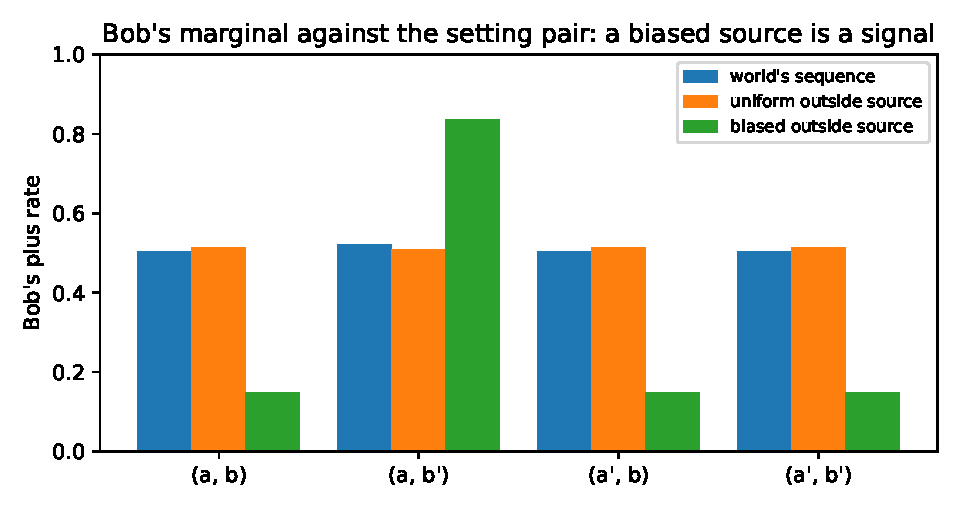
\includegraphics[width=0.85\linewidth]{figures/outside_source.pdf}
\caption{Bob's plus rate for each setting pair with the world's own sequence, a uniform outside source and a biased outside source, 1024 pairs each. Only the biased source moves Bob's rate with Alice's setting.}
\end{figure}

\section{What is new}\label{sec:new}

\begin{itemize}
\item One bounded-integer framework in which a classical phased field, a
finite quantum state, a hybrid local coupling and a shared-registry pair run
under identical computational conditions, so that the resource behind a
correlation can be isolated by changing one thing.
\item The null-notice mechanism: a local rule, sent through Links, that makes
the retarded conditional collapse of one excitation exact one Link later, with
an exact correction for notices that cross in flight, and a recorded causal
residual in between.
\item Bell's test as a measured causal anatomy: for each candidate, the
assumption of Bell's theorem it breaks is read off runs at fixed hidden
variable, and the bonded value is shown to be the registry's law pair by
pair, with its statistics.
\item A finite-integer statement of the no-signalling bound on the number
source, measured, and kept distinct from locality.
\end{itemize}

\section{What is not claimed}\label{sec:notclaimed}

\begin{itemize}
\item Not a derivation of quantum mechanics, the Born rule, the classical
limit or any configured law: the mixers, instruments, phase advance, the
$|p|/D$ rule, the cosine table and the singlet law in the registry are data,
measured to hold. Reproducing a configured law is a verification of the
implementation, not a prediction.
\item Not a local explanation of the Bell value: the bonded pair gives up
parameter independence, and no bookkeeping makes that local.
\item Born-rule consistency after null results is closed for one excitation
only; two carriers in one domain are outside the candidate by construction.
\item Back-action is a phase only; energy closure holds on the emission side
only; the field returns nothing to the wave.
\item Not a continuum or asymptotic result; every table is a finite lattice at
a finite number of ticks.
\item Not quantum electrodynamics, gravity, spin, statistics or many-body
dynamics, and not a claim that the lattice is a viable fundamental theory.
\item No prediction yet distinguishable from quantum mechanics with a
classical field.
\end{itemize}

What would make this a physics result: a local integer rule for several
excitations in one domain; the return path from field to wave; a dynamical
classical-limit experiment; a prediction that differs from quantum mechanics
with a classical field at a checkable scale. Beyond these, the code base
raises questions it cannot yet decide (the size of the universe, rotation
curves from a compressed closed dimension, redshift without recession, what
the integer sequence is); they are kept on a hypotheses page apart from the
results \cite{zenodo}.

\section*{Reproducibility}
Every table is produced by a checked-in harness that writes a summary with the
runtime source fingerprint; the archived version is \cite{zenodo}. Python 3.14,
no floating point in any physical module. The statistics of
Section~\ref{sec:bell} are produced by the Bell probe's sweep mode, and the
rates of Section~\ref{sec:causal} by its causal mode; both are pinned by tests.

\begin{thebibliography}{99}
\bibitem{fredkin1982} E. Fredkin and T. Toffoli, Conservative logic, Int. J. Theor. Phys. 21, 219 (1982).
\bibitem{thooft2016} G. 't Hooft, The Cellular Automaton Interpretation of Quantum Mechanics (Springer, 2016).
\bibitem{fhp1986} U. Frisch, B. Hasslacher and Y. Pomeau, Phys. Rev. Lett. 56, 1505 (1986).
\bibitem{succi2001} S. Succi, The Lattice Boltzmann Equation (Oxford, 2001).
\bibitem{bialynicki1994} I. Bialynicki-Birula, Phys. Rev. D 49, 6920 (1994).
\bibitem{meyer1996} D. A. Meyer, J. Stat. Phys. 85, 551 (1996).
\bibitem{arrighi2019} P. Arrighi, Natural Computing 18, 885 (2019).
\bibitem{rosenfeld1963} L. Rosenfeld, Nucl. Phys. 40, 353 (1963).
\bibitem{diosi1984} L. Di\'osi, Phys. Lett. A 105, 199 (1984).
\bibitem{oppenheim2023} J. Oppenheim, Phys. Rev. X 13, 041040 (2023).
\bibitem{grw1986} G. C. Ghirardi, A. Rimini and T. Weber, Phys. Rev. D 34, 470 (1986).
\bibitem{bassi2013} A. Bassi et al., Rev. Mod. Phys. 85, 471 (2013).
\bibitem{zurek2003} W. H. Zurek, Rev. Mod. Phys. 75, 715 (2003).
\bibitem{griffiths1984} R. B. Griffiths, J. Stat. Phys. 36, 219 (1984).
\bibitem{bombelli1987} L. Bombelli, J. Lee, D. Meyer and R. D. Sorkin, Phys. Rev. Lett. 59, 521 (1987).
\bibitem{bell1964} J. S. Bell, Physics 1, 195 (1964).
\bibitem{chsh1969} J. F. Clauser, M. A. Horne, A. Shimony and R. A. Holt, Phys. Rev. Lett. 23, 880 (1969).
\bibitem{jarrett1984} J. P. Jarrett, No\^us 18, 569 (1984).
\bibitem{shimony1986} A. Shimony, in Quantum Concepts in Space and Time, edited by R. Penrose and C. J. Isham (Oxford, 1986), p. 182.
\bibitem{hall2010} M. J. W. Hall, Phys. Rev. Lett. 105, 250404 (2010).
\bibitem{zenodo} A. Gonen, Universe24: a discrete simulator of local physical laws (Reality Theory), version 0.3.1, Zenodo (2026), doi:10.5281/zenodo.22738746 (concept DOI; the version DOI is listed on the record).
\end{thebibliography}

\end{document}
